\section{Program gto\char`_comparative\char`_map}
The \texttt{gto\char`_comparative\char`_map} creates a visualization for comparative maps.\\
For help type:
\begin{lstlisting}
./gto_comparative_map -h
\end{lstlisting}
In the following subsections, we explain the input and output paramters.

\subsection*{Input parameters}

The \texttt{gto\char`_comparative\char`_map} program needs an input file with the plot positions, respecting a defined structure.\\
The attribution is given according to:
\begin{lstlisting}
Usage: ./gto_comparative_map [options] [[--] args]                        
   or: ./gto_comparative_map [options]                                    
                                                                          
It creates a visualization for comparative maps.                          
                                                                          
    -h, --help            Show this help message and exit                 
                                                                          
Basic options                                                             
    <FILE>                Contigs filename with positions (.pos),         
                                                                          
Optional                                                                  
                                                                          
    -h                    Give this help,                                 
    -V                    Display version number,                         
    -v                    Verbose mode (more information),                
    -l <link>             Link type between maps [0;4],                   
    -w <width>            Chromosome width,                               
    -s <space>            Space between chromosomes,                      
    -m <mult>             Color id multiplication factor,                 
    -b <begin>            Color id beggining,                             
    -c <minimum>          Minimum block size to consider,                 
    -i                    Do NOT show inversion maps,                     
    -r                    Do NOT show regular maps,                       
    -o <FILE>             Output image filename with map,                 
                                                                          
Example: ./gto_comparative_map -o map.svg map.config 
\end{lstlisting}
%The input file needs to have the following structure:
%\begin{lstlisting}
%todo
%\end{lstlisting}
An example of such an input file is:
\begin{lstlisting}
#SCF    5000000 5000000
aaa     1       1000000 1       1000000 bbbb    3000000 4000000 3000000 4000000
bbb     1500000 2000000 1500000 2000000 cccc    1500000 2000000 1500000 2000000
aaa     2000000 3000000 2000000 3000000 bbbb    3000000 2000000 3000000 2000000
\end{lstlisting}

\subsection*{Output}
The output of the \texttt{gto\char`_comparative\char`_map} program is a executing report, and a svg plot with the maps.\\
Using the input above, an output example for this is the following:
\begin{lstlisting}
==[ PROCESSING ]====================
Printing plot ...
Found 2 regular regions. 
Found 1 inverted regions.
Done!                       

==[ STATISTICS ]====================
Total cpu time: 0 second(s).
\end{lstlisting}

In the Figure~\ref{fig:gtoComparativeMap} is represented the plot for the execution above.

 \begin{figure}[!h]
  \centering
  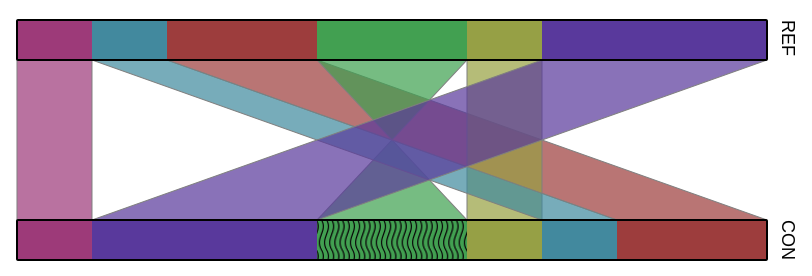
\includegraphics[scale=0.6]{./images/gto_comparative_map.png}
  \caption{\texttt{gto\char`_comparative\char`_map} execution plot.}
  \label{fig:gtoComparativeMap}
 \end{figure}